\chapter{Аналитический раздел}
\label{cha:analysis}

В данном разделе проводится анализ и выбор методов создания, рендера сложных моделей.  

\section{Анализ методов создания сложных моделей}

Моделирование твердого тела - это последовательный набор принципов математического и компьютерного моделирования трехмерных твердых тел \cite{lec:modeling_schemes}. 
На данном этапе стоит рассмотреть существующие схемы представления твердотельной модели.

\subsection{Клонирование примитивов}
Схема основана на понятии семейств объектов: выделяются определённые члена семейства, отличающиеся несколькими параметрами друг от друга. 
С помощью операций поворота, масштабирования (см. рис. \ref{fig:primitive_instancing}) можно изменять объект.
\begin{figure}
  \centering
  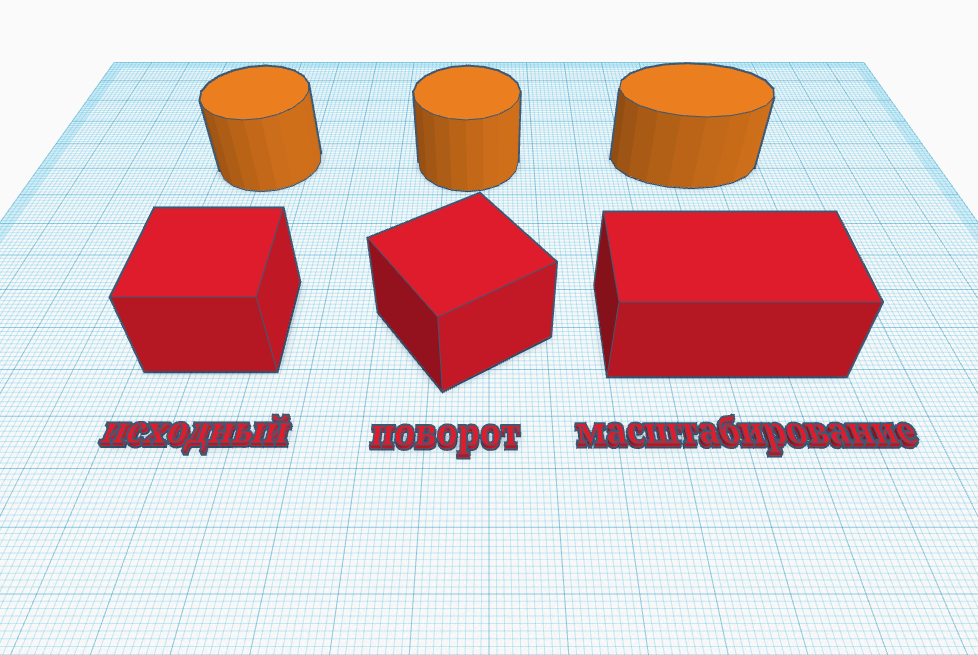
\includegraphics[scale=0.3]{inc/img/primitive_instancing}
  \caption{Пример клонирования примитивов на примере куба и цилиндра}
  \label{fig:primitive_instancing}
\end{figure}

\clearpage
Каждое семейство объектов называется общим примитивом, а отдельные объекты называются примитивными экземплярами.
Например, семейство болтов является общим примитивом, а отдельный болт, заданный определенным набором параметров (см. рис. \ref{fig:bolt}), является примитивным экземпляром.
\begin{figure}
  \centering
  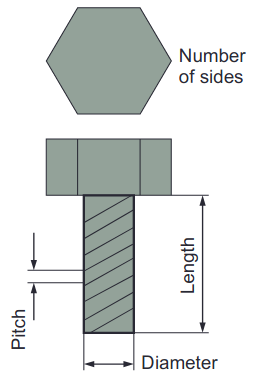
\includegraphics[scale=0.6]{inc/img/bolt}
  \caption{Болт задан параметрами: количество сторон головы, шаг резьбы, длина, диаметр}
  \label{fig:bolt}
\end{figure}

Особенности: 
\begin{itemize}
\item невозможно создать сложный объект, с помощью объединения экзепляров.
\end{itemize}

Минусы:  
\begin{itemize} 
\item cложность написания алгоритмов для вычисления свойств представленных твердых тел из - за уникальности каждого примитива, 
следовательно, обобщить обработку невозможно.
\end{itemize}

Плюсы:
\begin{itemize}
  \item способ хорош, если требуется только представление определённого семейства моделей.
\end{itemize}

Чтобы решить поставленную задачу, нужна схема, с помощью которой можно не зависеть от типа модели: его формы, параметров.

Рассмотрев схему можно заключить, что она не подходит для решения задачи, так как возникает потребность в подробном описании
всех свойств определённого семейства, а учитывая потребность в составных телах, сделать для них это будет проблематично.

\subsection{Нумерация пространственного заполнения} \label{numeric_scheme}
Cхема из себя представляет список-сетку пространственных ячеек, занятых твердым телом.
Ячейки (воксели) представляют собой кубы фиксированного размера (см. рис. \ref{fig:spatial_occupacy}) и расположены в заданной пространственной сетке. 
3D объект представляет собой список закрашенных вокселей.
\begin{figure}
  \centering
  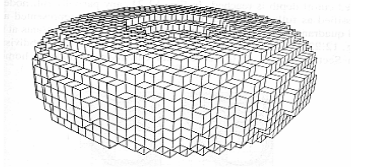
\includegraphics[scale=1.2]{inc/img/spatial_occupacy}
  \caption{Пример представления тора методом нумерации пространственного заполнения}
  \label{fig:spatial_occupacy}
\end{figure}

Каждая ячейка может быть представлена ​​координатами одной точки, например центроида ячейки.

Обычно устанавливается определенный порядок сканирования, и соответствующий упорядоченный набор координат называется пространственным массивом.

Пространственные массивы являются однозначными и уникальными твердыми представлениями, но слишком подробны для использования в качестве «основных» представлений \cite{lecture_solid_modeling}.

Минусы:  
\begin{itemize} 
\item затраты памяти высоки;
\item каждая ячейка хранит информацию о занятости, цвете, плотности и др.;
\item разрешение ограничено размером и формой вокселя.
\end{itemize}

Плюсы:
\begin{itemize}
  \item простая структура данных;
  \item однозначное представление.
\end{itemize}

Данная схема удобна с точки зрения простоты и точности представления, однако, структурно состоит из кубических форм,
для рендера, например, сферы, потребуется дополнительно сглаживать края, что накладывает дополнительную вычислительную нагрузку. 

Также для нас избыточно хранения в каждой ячейке информации о её состоянии.
Самостоятельное использование метода нецелесообразно, однако совместно с другими методами, можно использовать преимущество грубой апроксимации, для
повышения точности изображаемого тела. 
\subsection{Sweeping}
Эта схема позволяет создавать 3D модели из 2D с помощью движения по заданной траектории: вокруг оси (см. рис. \ref{fig:sweeping}), относительно граней и др. \cite{lecture_solid_modeling}.


\begin{figure}
  \centering
  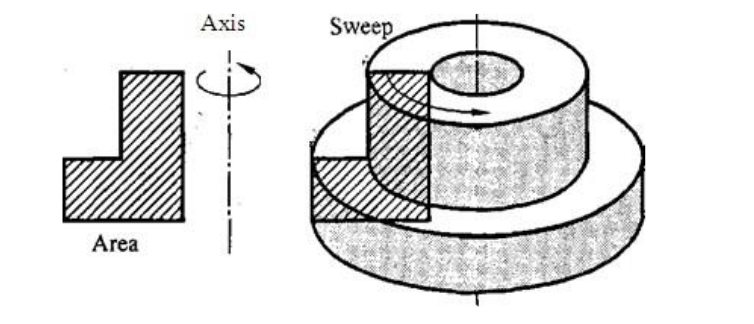
\includegraphics[scale=0.6]{inc/img/sweeping}
  \caption{Тело образовано вращением вокруг оси}
  \label{fig:sweeping}
\end{figure}

Плюсы:
\begin{itemize}
  \item простые формы удобно задавать через плоские фигуры;
  \item может использоваться для быстрого удаления материала внутри тела (см. рис. \ref{fig:sweeping_delete}).
\end{itemize}
\clearpage
\begin{figure}
  \centering
  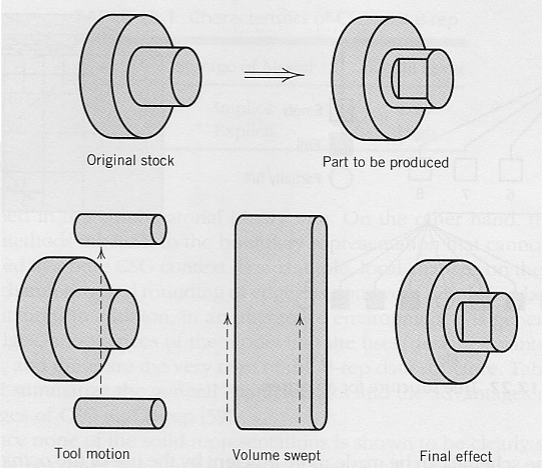
\includegraphics[scale=0.6]{inc/img/sweeping_delete}
  \caption{Удаление материала с помощью sweeping}
  \label{fig:sweeping_delete}
\end{figure}

Минусы:  
\begin{itemize}
\item необходимо задать траекторию движения 2D объекта, что проблематично для тел, имеющих сложную форму.
\end{itemize}
\subsection{Октантное дерево}
Схема является улучшением воксельного представления. Каждый узел октантного дерева соответствует некоторому кубу в трехмерном пространстве, для которого определяется принадлежность модели.
У каждого корня дерева есть 8 потомков, т.е куб делится на 8 равных частей (см. рис. \ref{fig:octree}).
\begin{figure}
  \centering
  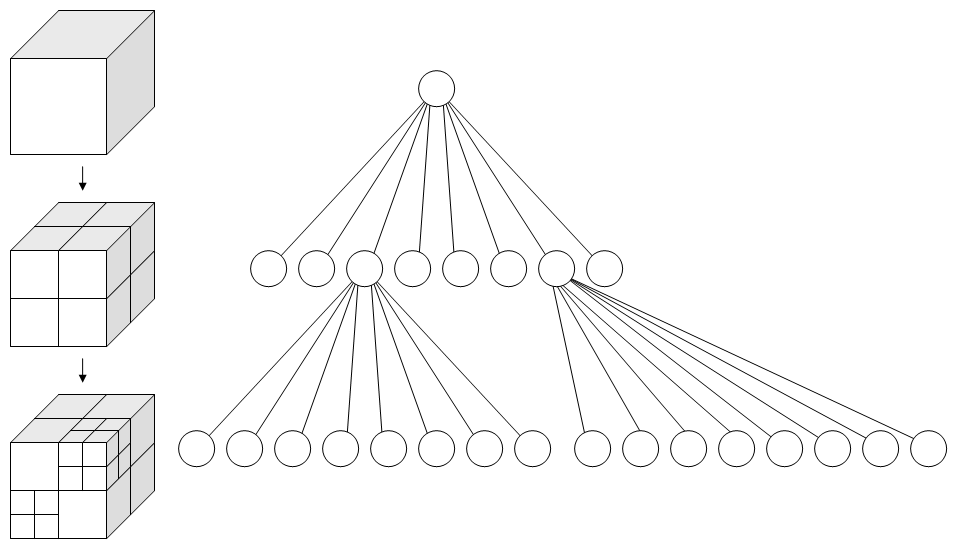
\includegraphics[scale=0.4]{inc/img/octree}
  \caption{Слева: Рекурсивное разделение куба на октанты. Справа: Соответствующее октодерево.}
  \label{fig:octree}
\end{figure}

Метод позволяет устранить недостаток метода \ref{numeric_scheme}, связанный с хранением большого количества данных, сохраняя информацию только об используемых частях модели.
Однако в сравнении с другими методами, памяти расходуется всё так же много. 

Обычно, используется в сферах, требующих точное представление, например, в медицине \cite{octree}.

Минусы:  
\begin{itemize} 
\item возможное деления примитива ребрами кубов дерева, что снижает эффективность;
\item вывод всех объектов, находящихся в поле камеры, но на самом деле в конечном счёте невидимых.
\end{itemize}

\subsection{Граничное представление(BREP)}
Способ представления модели с помощью границ. Замкнутая 2D-поверхность определяет 3D-объект.

Суть BRep-представления заключается в том, что твердое тело описывает замкнутая пространственная область,
ограниченная набором элементарных поверхностей (граней) с общими образующими  контурами (ребрами) на границе поверхностей (см. рис. \ref{fig:brep})
и признаком внешней или внутренней стороны поверхности.
\begin{figure}
  \centering
  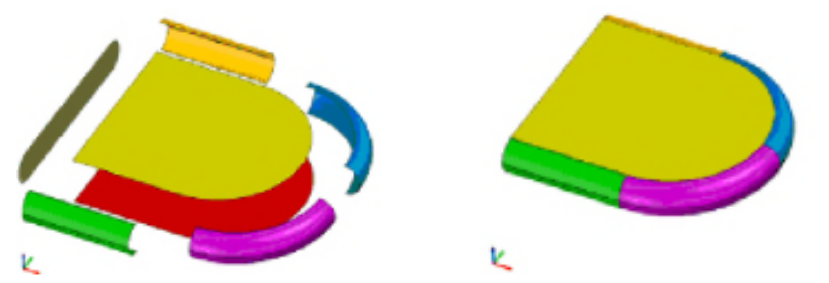
\includegraphics[scale=0.6]{inc/img/brep}
  \caption{BRep-представление простых твердых тел}
  \label{fig:brep}
\end{figure}

Данный способ проектирования в приложениях САПР является наиболее распространненным, 
однако имеет недостатки, из-за которых возникает проблема визуализации результата \cite{main_modeling}.


Минусы: 
\begin{itemize} 
\item высокие затраты памяти;
\item когда объект необходимо отрендерить объект требует слишком много вычислительной мощности;
\item для сложных объектов возникают трудности получения математических формул их описывающих.  
\end{itemize}

Плюсы:
\begin{itemize}
  \item подходит не только для твердых тел с плоскими гранями, но и для криволинейных объектов с замкнутыми криволинейными гранями или краями.
  \item позволяет проводить различные вычисления, требующие точность, благодаря хранению информации о всех составляющих модели.
\end{itemize}

\subsection{Конструктивная сплошная геометрия(CSG)}\label{csg}
Данный способ представления основан комбинирования примитивов посредством логических операций,
что позволяет создавать сложные модели на основе простых с помощью:
\begin{itemize}
  \item объединения;
  \item пересечения;
  \item разности.
\end{itemize}

Любое составное тело может быть описано в виде традиционного уравнения из булевых функций,
в котором аргументами являются либо элементарные тела, либо другие составные тела.
Это представление называют деревом построений (см. рис. \ref{fig:csg_tree}) \cite{main_modeling}.
\clearpage
\begin{figure}
  \centering
  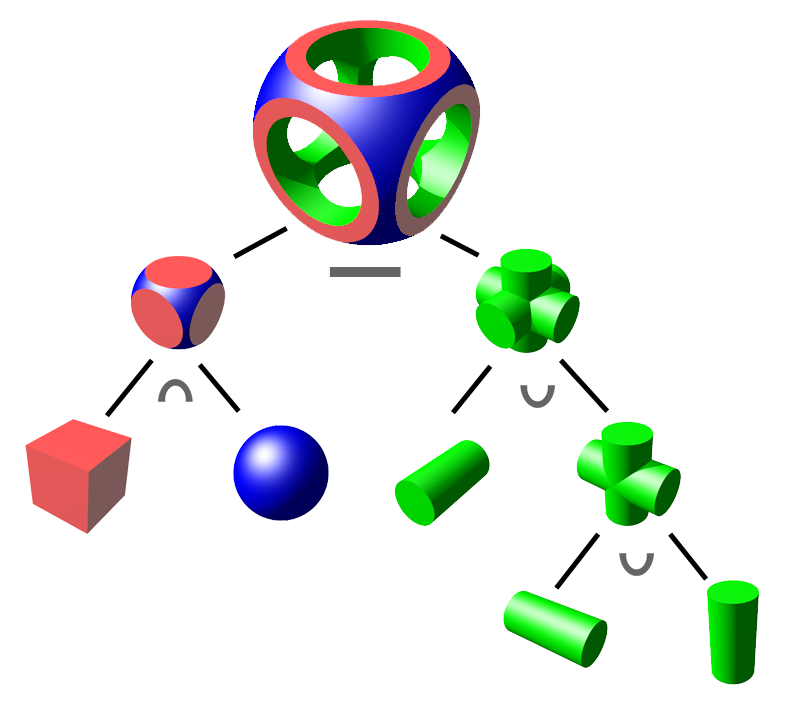
\includegraphics[scale=0.3]{inc/img/csg_tree}
  \caption{Сложный объект может быть представлен двоичным деревом, 
  где «листья» — это объекты, а узлы — операции. 
  ( пересечение, объединение, −  - разность)}
  \label{fig:csg_tree}
\end{figure}

Особенности:  
\begin{itemize}
  \item При использовании логических операций нужно иметь ввиду, что комбинирование может привести к вырождению твердого тела в плоское. 
\end{itemize}
\subsection{Сравнение схем}
Сравнивая схемы, предлагается разобрать следующие критерии:
\begin{enumerate}
  \item Лаконичность, т.е сколько памяти компьютера занимает модель (+ значит мало, - иначе: модель хранит не всегда используемую информацию), для решения задачи требуется минимальный расход;
  \item Эффективность, т.е насколько много времени необходимо для создания, исследования или изменения формы модели;
  \item Уникальность, т.е получить модель можно только одним способом;
  \item Однозначность, т.е вместе с моделью хранятся данные, которых достаточно для осуществления геометрических расчётов;
  \item Хранение истории преобразования модели, чтобы у пользователя была возможность вернуться к предыдущему шагу моделирования тела без применения афинных преобразований и дополнительных вычислений;
  \item Практичность, т.е создание модели без введения дополнительных параметров, поддерживая удобство использования.
\end{enumerate}
Разбор рассмотренных по критериям методов представлен в таблице 1.1.
\begin{table}[ht]
  \small
  \caption{Сравнительная таблица схем представления твёрдого тела}
  \begin{tabular}{|r|c|c|c|c|c|c|l|}
  \hline
  Методы&Лак-ть&Эф-ть&Ун-ть&Одноз-ть&История&Прак-ть\\
  \hline
  Клонирование примитивов  &-&+&-&+&-&-\\
  Нумер-я простр-го заполн. &-&-&+&+&-&-\\
  Октантное дерево & +& -& + & + & - & -\\
  BREP & -  & + & + & + & - & -\\
  Sweeping  & +  & - & - & + & -& -\\
  CSG  & + & + & - & + & + & + \\
  \hline
  \end{tabular}
  \label{tab:schemes}
\end{table}

После рассмотрения схем представления предлагается использовать CSG как наиболее подходящий метод создания моделей.
Представление  твердых  тел  в  виде  дерева  построений (листья - примитивы, узлы - результат операции) удобно также с точки зрения 
модификации объекта и организации пользовательского интерфейса, обеспечивающего наглядный и быстрый доступ к любому  элементу,
входящему  в  описание  геометрии тела. Остальные схемы требуют дополнительную информацию, которая необходима для обработки и создания моделей, 
но для решения задачи она не является необходимостью.


\clearpage


\section{Анализ методов рендера модели}
После того, как был выбран способ создания твердотельной модели, следует изучить методы рендера.  

Рендеринг (англ. rendering — «визуализация») "--- термин, обозначающий процесс получения изображения по модели с помощью компьютерной программы \cite{article:rendering}.\\
Рассмотрим возможные варианты:

\subsection{Растеризация}
Растеризация "--- это процесс получения растрового изображения \cite{article:rasterization}.\\
Растровое изображение - это изображение, представляющее собой сетку пикселей — цветных точек (обычно прямоугольных) на мониторе, 
бумаге и других отображающих устройствах \cite{article:rastr_image}.\\  
Технология основана на обходе лучем вершин треугольника (см. рис. \ref{fig:raster_scene}), 
который остаётся самим собой даже после попадания из трехмерного пространства в двухмерное.\\
\begin{figure}
  \centering
  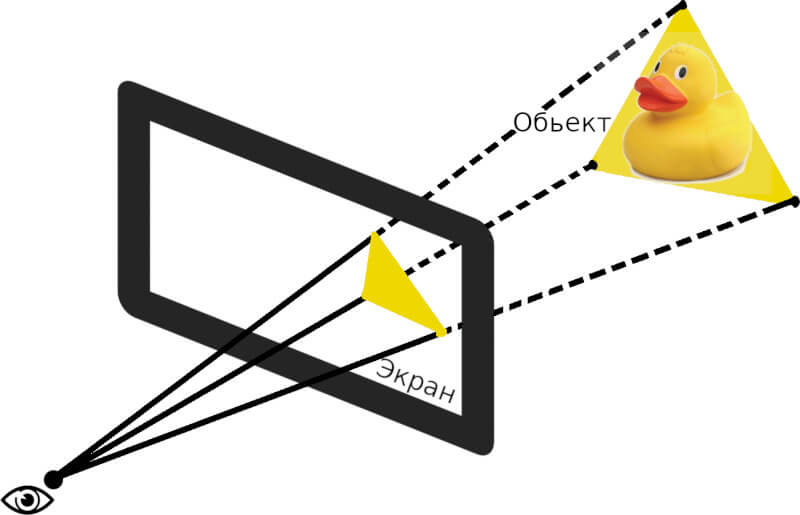
\includegraphics[scale=0.4]{inc/img/raster_scene}
  \caption{Схематическое отображение предмета на экран}
  \label{fig:raster_scene}
\end{figure}

\clearpage
Каждая точка каждого объекта в трехмерном пространстве переводится в точку на экране (см. рис. \ref{fig:raster_projection}),
а затем точки — заданные в модели треугольники — соединяются и получается изображение исходного объекта.\\

\begin{figure}
  \centering
  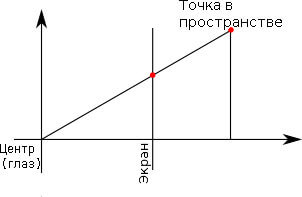
\includegraphics[scale=0.8]{inc/img/raster_projection}
  \caption{Проецирование точки из пространства на плоскость экрана, вид сбоку}
  \label{fig:raster_projection}
\end{figure}

Преимущества и недостатки:
\begin{itemize}
  \item изображение может быть "угловатым"(ступенчатым) - нуждается в сглаживании;
  \item требует больших вычислительных ресурсов - могут использоваться миллионы полигонов для всех моделей объектов сцены и примерно 8 миллионов пикселей на дисплее 4K,
  и каждый кадр или изображение, отображаемое на экране, обычно обновляется на дисплее от 30 до 90 раз в секунду \cite{nvidia:rastr};
  \item каждый пиксель обрабатывается много раз;
  \item 3D модель должна быть описана из примитивов, следовательно, составные модели обрабатывать ресурсозатратно, т.к нужно разбить его на примитивы, обычно, треугольники.
  \item современные компьютеры оптимизированы для рендеринга растровых изображений, благодаря чему этот процесс достаточно быстрый, однако, 
  как было сказано выше, с ростом сложности изображения, возрастают время рендера и потребности к ресурсам.
\end{itemize}
\clearpage

\subsection{Трассировка лучей}
\subsubsection{RayCasting}
Ray-casting (рус. — бросание лучей) "--- это технология, которая преобразует набор данных в 3D проекцию путем «бросания лучей» из точки обзора по всей области видимости. 

Основная идея -  испускать лучи из «глаз» наблюдателя, один луч на пиксель, и находить самый близкий объект,
который блокирует путь распространения этого луча (см. рис. \ref{fig:raycast_ex}). 
Последующая обработка преломленных от объекта лучей в этом методе отсутствует.
Используя свойства материала и эффект света в сцене, алгоритм бросания лучей может определить затенение данного объекта \cite{article:raycasting}.

\begin{figure}
  \centering
  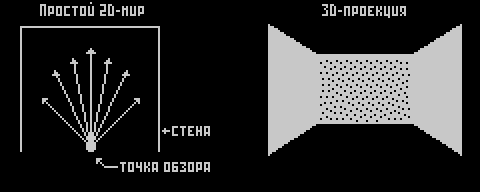
\includegraphics[scale=0.8]{inc/img/raycast_ex}
  \caption{На рисунке показано, как бросание преобразует что-то двумерное во что-то почти что трехмерное.}
  \label{fig:raycast_ex}
\end{figure}

Метод использовался при создании игр в конце прошлого века, такую графику иногда называют "псевдо 3D" или "2.5D". 

Из простоты алгоритма вытекает ряд ограничений, сказывающихся на качестве результата (см. рис. \ref{fig:raycast_game}), ведь на деле это
всего лишь трёхмерная проекция плоского изображения.
Ограничения алгоритма на примере применения в игровом мире \cite{article:who_to_work_raytrace}: 
\begin{enumerate}
  \item все доступное в игре пространство — это комната с прямоугольными (чаще квадратными) стенами;
  \item нет лестниц, лифтов, любого вида спусков и подъемов;
  \item потолок везде имеет одинаковую высоту;
  \item нет других трехмерных объектов, кроме стен, пола и потолка, все остальные объекты - двумерные изображения, расположенные в трехмерном пространстве.
\end{enumerate}
% На рисунке \ref{fig:raycast_game} изображена сцена из компьютерной игры $90$-х годов $XX$ века, демонстрирующая графические возможности алгоритма. 
\begin{figure}
  \centering
  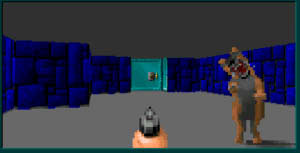
\includegraphics[scale=1]{inc/img/raycast_game}
  \caption{Сцена из Wolfenstein 3D. Картинка делится на прямоугольные блоки. Объекты (оружие) и враги (собака) — это просто прозрачные растровые изображения, которые масштабированы и отрисованы поверх заднего фона.}
  \label{fig:raycast_game}
\end{figure}

Минусы:
\begin{itemize}
  \item в результате рендера получается изображение среднего-плохого качества, в сравнении с остальным методами;
  \item геометрические ограничение на обрабатываемую поверхность(только простые фигуры);
  \item эффективен для объектов, у которых нет больших затрат на вычисление пересечения луча.
\end{itemize}

Плюсы:  
\begin{itemize}
  \item прост в реализации;
  \item нетребователен;
  \item изображение генерируется "на лету".
\end{itemize}
\subsubsection{RayTracing}
Трассировка лучей (англ. Ray Tracing) "--- это технология отрисовки трехмерной графики, симулирующая физическое поведение света \cite{article:who_to_work_raytrace}.\\
Принцип работы трассировки лучей:\\
поскольку все существующие трехмерные модели собраны из треугольников, 
нужно было обязательно сохранить обратную совместимость - для этого проверяется случай столкновения луча не со стеной, а с треугольником.
Рассмотрим его.
\begin{eqndesc}
Пусть вершины треугольника обозначены через $V_0$, $V_1$, $V_2$.
Векторы двух его рёбер обозначены как $A$, $B$ и заданы формулами \ref{eq:vector_triangle_a} и \ref{eq:vector_triangle_b}:\\
\begin{equation} \label{eq:vector_triangle_a}
  A = V_1 - V_0
\end{equation}
\begin{equation} \label{eq:vector_triangle_b}
  B = V_2 - V_0
\end{equation}
Определим луч $P$ с помощью параметрической формы уравнения \ref{eq:param_line}:
\begin{equation} \label{eq:param_line}
  P = R_0 + t \cdot R_d
\end{equation}
где $R_0$ "--- начальная точка луча, $R_d$ "--- направление луча, $t$ "--- расстояние вдоль луча, на которое попала точка\\
С другой стороны, точка пересечения имеет координаты $u$, $v$ в плоскости треугольника. Приравняв
уравнение луча $P$ и плоскости в точке $u$, $v$ (см. формулу \ref{eq:point_in_triangle}), можно найти пересечение:\\
\begin{equation} \label{eq:point_in_triangle}
  P = V_0 + u \cdot A + v \cdot B
\end{equation} 
Таким образом, составив систему из трех уравнений \ref{eq:system_for_coords} для координат $x, y, z$ и решив её для $t, u, v$, необходимо 
проанализировать определитель. Если он ненулевой(луч не параллелен плоскости), а $t >= 0$ и $u, v, u + v$ лежат в диапазоне от $0\dots1$, 
то $P$ находится внутри треугольника и поиск столкновения завершается.
 \\
\end{eqndesc}
\clearpage
\begin{eqndesc}
\begin{equation} \label{eq:system_for_coords}
\begin{aligned}
\begin{cases}
  R_0.x + t \cdot R_d.x = V_0.x + u \cdot A.x + v \cdot B.x \\
  R_0.y + t \cdot R_d.y = V_0.y + u \cdot A.y + v \cdot B.y \\
  R_0.z + t \cdot R_d.z = V_0.z + u \cdot A.x + v \cdot B.z \\
\end{cases}
\end{aligned}
\end{equation}
\end{eqndesc}

Особенность же трассировки лучей состоит в том, что на одном треугольнике серия вычислений не заканчивается, 
ведь некоторые поверхности могут быть зеркальными или просто блестеть. 
В таком случае луч не останавливается, а отражается от этого треугольника и снова ищет себе цель до тех пор, пока не вернётся в начальную точку, 
или не превысит максимальное число отражений.
Вся сложность алгоритма позволяет получить качественное изображения, в сравнении с полученным в результате растеризации (см. рис. \ref{fig:raster_vs_tracer}).

  \begin{figure}
  \centering
  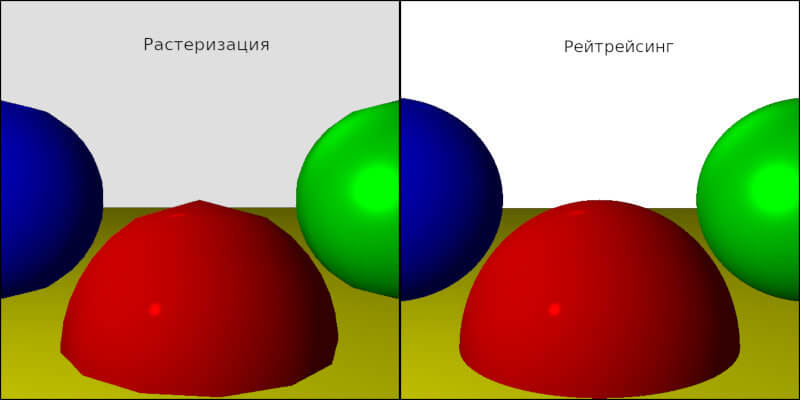
\includegraphics[scale=0.5]{inc/img/raster_vs_tracer}
  \caption{Сравнение растеризации и трассировки лучей}
  \label{fig:raster_vs_tracer}
\end{figure}
\clearpage

Плюсы: 
\begin{itemize}
  \item возможность рендеринга гладких объектов без аппроксимации их полигональными поверхностями (например, треугольниками);
  \item вычислительная сложность метода слабо зависит от сложности сцены;
  \item отсечение невидимых поверхностей, перспектива и корректное изменения поля зрения являются логическим следствием алгоритма.
\end{itemize}

Однако, главным недостатком метода является производительность. 
Метод трассирования лучей каждый раз начинает процесс определения цвета пикселя заново, 
рассматривая каждый луч наблюдения в отдельности. Что даёт изображению реалистичность, решает задачу отражения, но требует много ресурсов.\\
Следует рассмотреть модификацию данного алгоритма.  
\clearpage

\subsubsection{RayMarching}
Марширование лучей (англ. RayMarching) - разновидность алгоритма трассировки лучей.

Raymarching похож на традиционную трассировку лучей (raytracing) тем, что луч в сцену испускается для каждого пикселя. 
В трассировщике лучей есть набор уравнений, определяющих пересечение луча и рендерящихся объектов. 
Raymarching предлагает другой метод решения задачи пересечения луча и объекта, не пытается вычислить персечение аналитически.
При нём происходит смещение текущего положения вдоль луча, пока не будет найдена точка, пересекающая объект. 
Эта операция является относительно простой и малозатратной, гораздо более практичной в реальном времени.\\
Однако, этот способ не точно находит пересечение (см. рис. \ref{fig:raymarch_2}). 
\begin{figure}
  \centering
  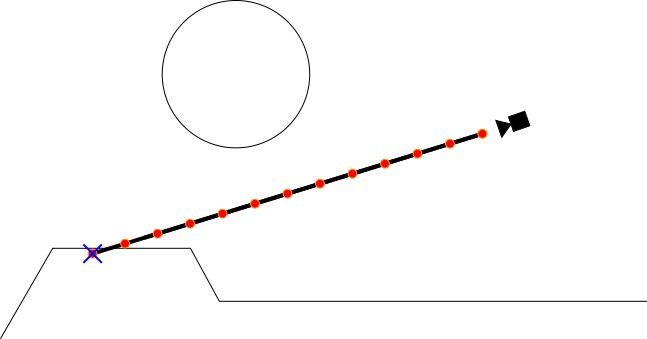
\includegraphics[scale=0.8]{inc/img/raymarch_2}
  \caption{Простейшая реализация метода с фиксированным интервалом шага. Красными точками обозначены все сэмплируемые точки.}
  \label{fig:raymarch_2}
\end{figure}

\subsubsection{Функция поля расстояний} \label{anl:sdf}
Реализация, разобранная выше, вполне достаточна для множества областей применения, например, объёмных и прозрачных поверхностей. 
Однако для непрозрачных объектов можно ввести ещё одну оптимизацию. 
Для этой оптимизации требуется использование полей расстояний со знаком. 

Поле расстояний (signed distance fields) "" --- это функция, получающая на входе точку и возвращающая кратчайшее расстояние от этой точки до поверхности каждого объекта в сцене. 
SDF возвращает отрицательное число, если точка находится внутри объекта. 

Этот инструмент позволяет нам ограничить количество шагов при движении вдоль луча (см. рис. \ref{fig:raymarch_3}),
что увеличивает эффективность метода.\\
\begin{figure}
  \centering
  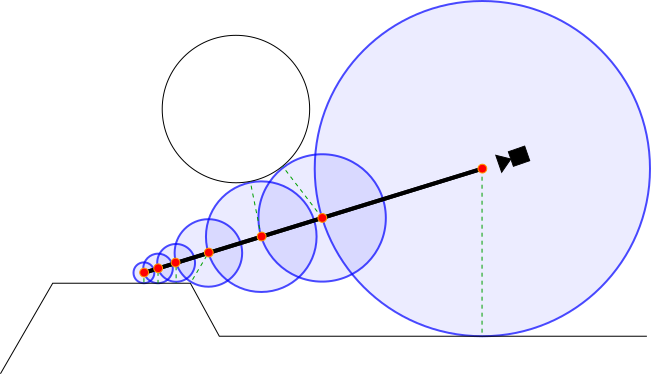
\includegraphics[scale=0.8]{inc/img/raymarch_3}
  \caption{Визуализация метода, с использованием SDF. Красными точками показаны все сэмплируемые точки. Синими кругами показаны области, которые гарантированно не содержат объектов (потому что они находятся в результатах функции поля расстояний). Пунктирными зелёными линиями показаны истинные кратчайшие векторы между каждой сэмплируемой точкой и сценой.}
  \label{fig:raymarch_3}
\end{figure}

Описание алгоритма \cite{article:who_to_work_3d}: 
\begin{itemize}
  \item для пикселя на экране определяется расстояние до ближайшего объекта;
  \item это расстояние определяет радиус на который можно пустить луч;
  \item пускаем луч;
  \item для конечной точки луча предыдущие пункты повторяются до тех пор пока следующий радиус не станет достаточно маленьким, 
  что будет означать столкновение с объектом. Или же радиус может начать стабильно увеличиваться, если луч прошел мимо всех объектов.
\end{itemize}
Плюсы:
\begin{itemize}
  \item решает проблему производительность трассировки лучей, работает быстро;
  \item подходит для рендера поверхностей, для которых сложно или невозможно вычислить пересечение аналитически;
  \item используя SDF можно ускорить рендеринг до реального времени;
  \item подходит для графического процессора, так как каждый пиксель можно рассчитать независимо;
  \item качество изображения сопоставимо с полученным при трассировке лучей.
\end{itemize}
Минусы:
\begin{itemize}
  \item пересечение вычисляется неточно, с некоторой погрешностью;
\end{itemize}
\clearpage
\subsubsection{Сравнение методов}
Сравнивая рассмотренные методы рендеринга, предлагается разобрать следующие критерии:
\begin{enumerate}
  \item качество;
  \item эффективность, т.е насколько много времени необходимо для рендера модели;
  \item выполнение в режиме реального времени;
  \item точность, т.е обработка истинных границ обрабатываемой модели;
\end{enumerate}
Разбор рассмотренных по критериям методов представлен в таблице \ref{tab:render}.
\begin{table}[ht]
  \caption{Сравнительная таблица методов рендеринга}
  \begin{tabular}{|r|c|c|c|c|}
  \hline
  Методы & Качество & Эффективность & Реал.время & Точность\\
  \hline
  Растеризация & - & + & + & + \\
  RayCasting & - & + & + & +\\
  RayTracing & + & - & - & +\\
  RayMarching & + & + & + & -\\
  \hline
  \end{tabular}
  \label{tab:render}
\end{table}

В данном разделе были рассмотрены методы рендера модели. Учитывая метод, выбранный в предыдущем  разделе, а также анализ в текущем,
можно сказать, что алгоритм raymarching наиболее привлекателен для рендера конструктивной сплошной геометрии,
в такой связке можно получить качественное изображение при его отрисовке в реальном времени. 
Один недостаток, это вычисление границ объекта с некоторой погрешностью, но остальные плюсы метода затмевают его.  
\section{Преобразования и визуализация}
В данном пункте рассматриваются средства для преобразования модели и 
придания ей трехмерного вида.
\subsection{Шейдеры}
Шейдер -  компьютерная программа, предназначенная для исполнения процессорами видеокарты (GPU) \cite{article:shaders}.

В разрабатываемом приложении использование шейдеров необходимо для придания изображению трехмерного вида, 
используя тени, освещение. 
Для этого предназначены фрагментный и вершинный шейдеры.
\subsubsection{Вершинные шейдеры} \label{anl:vert_shader}
Вершинный шейдер получает вершину из списка вершин и отображает ее в пространстве.
Вершинному шейдеру передаются следующие данные:
\begin{itemize}
  \item матрица модели;
  \item матрица вида;
  \item матрица проекции.
\end{itemize}

Матрица модели:

Необходима для перехода от пространства модели (все вершины определены относительно центра модели) 
в мировое пространство (все вершины определены относительно центра мира).

Матрица вида:

Необходима для перемещения сцены относительно камеры. В реальном мире происходит перенос самой камеры, точки обзора. 
В компьютерной графике более просто и удобно переместить сцену относительно камеры, тем самым в результате 
получить перемещение камеры относительно сцены.  

Матрица проекции:

Эта матрица используется для представления перспективы камеры. Умножение координат на данную матрицу 
позволяет сопоставить вершину с перспективой камеры, учитывая ее соотношения сторон, поля обзора
и самого дальнего и ближайшего объекта, который виден. 

Для преобразования координат выполняются следующие действия:
\begin{enumerate}
  \item положение вершины умножается на матрицу модели, чтобы определить, где эта вершина находится относительно центра модели в сцене;
  \item результат умножается на матрицу вида, чтобы определить, где расположена вершина относительно камеры;
  \item результат второй операции умножается на матрицу проекции, чтобы определить, где находится вершина в перспективе камеры. 
\end{enumerate}
\subsubsection{Фрагментные шейдеры}
Фрагментный шейдер работает с пикселями объекта и управляет цветом пикселя.
Выполнение фрагментного шейдера в графическом конвейере происходит после вершинного, следовательно, никак не влияет на координаты вершины,
он влияет только на цветовую составляющую, преобразуя вершины уже в пиксели или фрагменты.

Помимо придания трехмерного вида, к моделям следует применять операции, 
которые позволяют изменять их положение и ориентацию. 
\subsection{Матрицы преобразования}
Для преобразования тела в пространстве используются операции:
\begin{itemize}
  \item перемещения;
  \item масштабирования;
  \item поворота.
\end{itemize}

Осуществляются преобразования с помощью матриц \ref{tab:matrix}. 
\begin{table}[ht]
\caption{Таблица преобразований}
\begin{tabular}{|l|c|l|}
\hline
Преобразование & Матрица & Формула\\
\hline
Перемещение      & $\begin{pmatrix}
    1  & 0  & 0  & 0 \\
    0  & 1  & 0  & 0 \\
    0  & 0  & 1  & 0 \\
    dx & dy & dz & 1
  \end{pmatrix}$  & $\begin{cases}
    x_1=x+dx \\
    y_1=y+dy \\
    z_1=z+dz
  \end{cases}$  \\
\hline
Масштаб - е  & $\begin{pmatrix}
    k_x & 0   & 0   & 0 \\
    0   & k_y & 0   & 0 \\
    0   & 0   & k_z & 0 \\
    0   & 0   & 0   & 1
  \end{pmatrix}$ & $\begin{cases}
    x_1=k_x+(1-k_x)x_m \\
    y_1=k_y+(1-k_y)y_m \\
    z_1=k_z+(1-k_z)z_m
  \end{cases}$ \\
\hline
Поворот OX & $\begin{pmatrix}
    1 & 0           & 0          & 0 \\
    0 & \cos\theta  & \sin\theta & 0 \\
    0 & -\sin\theta & \cos\theta & 0 \\
    0 & 0           & 0          & 1
  \end{pmatrix}$ & $\begin{cases}
    x_1=x                                       \\
    y_1=y_c+(y-y_c)\cos\theta-(z-z_c)\sin\theta \\
    z_1=z_c+(y-y_c)\sin\theta+(z-z_c)\cos\theta
  \end{cases}$ \\
\hline
Поворот OY & $\begin{pmatrix}
    \cos\theta & 0 & -\sin\theta & 0 \\
    0          & 1 & 0           & 0 \\\sin\theta&0&\cos\theta&0 \\
    0          & 0 & 0           & 1
  \end{pmatrix}$ & $\begin{cases}
  x_1=x_c+(x-x_c)\cos\theta+(z-z_c)\sin\theta \\
  y_1=y \\
  z_1=z_c-(x-x_c)\sin\theta+(z-z_c)\cos\theta
  \end{cases}$ \\
\hline
Поворот OZ & $\begin{pmatrix}
    \cos\theta  & \sin\theta & 0 & 0 \\
    -\sin\theta & \cos\theta & 0 & 0 \\
    0           & 0          & 1 & 0 \\
    0           & 0          & 0 & 1
  \end{pmatrix}$ & $\begin{cases}
    x_1=x_c+(x-x_c)\cos\theta-(y-y_c)\sin\theta \\
    y_1=y_c+(x-x_c)\sin\theta+(y-y_c)\cos\theta \\
    z_1=z
  \end{cases}$ \\
\hline
\end{tabular}
\label{tab:matrix}
\end{table}
\clearpage

Исходные координаты объекта умножаются на одну или несколько матриц, в результате чего
объект перемещается/масштабируется/поворачивается, в зависимости от примененных преобразований.  
Помимио этого, матрицы позволяют перевести координаты модели в мировые, переместить сцену относительно камеры, настроить перспективу.

В данном пункте были рассмтрены средства для преобразования модели - матрицы преобразования, а также
для преобразования плоского изображения в трехмерный вид - шейдеры.
\section{Аппаратная обработка}
В данном разделе предлагается рассмотреть аппаратную составляющую рендеринга.
Есть 2 основных варианта: рендеринг на центральном и графическом процессорах.
Они имеет много общего, но существуют различия,
которые оказывают огромное влияние на скорость и качество изображения. 
Рендеринг на базе ЦП является традиционным способом и широко используется. Напротив, рендеринг с помощью графических процессоров 
с годами становится все более популярным в сообществе благодаря быстроразвивающемуся миру технологий.
Рассмотрим подробнее каждый из процессоров.
\subsection{CPU}
CPU "--- центральный процессор, это основной компонент компьютера, обрабатывающий инструкции. 
Он выполняет вычисления, действия, запускает программы, включая рендеринг. 
Центральный процессор постоянно принимает ввод от пользователя или активных программ, затем обрабатывает данные и выдает вывод, который может быть сохранен приложением или отображен на экране \cite{article:cpu_gpu}.
\subsection{GPU}
GPU "--- графический процессор. Разработан для параллельной обработки трудоёмких вычислительных задач. 
Графический процессор используется в широком спектре приложений, ускоряющих рендеринг 3D-графики.
Кроме того, этот микропроцессор также используется для разгрузки некоторых задач с центрального процессора, что заставляет компьютер работать быстрее \cite{article:cpu_gpu}.
\subsection{Сравнение процессоров}
Рассмотрим различия процессоров приминительно к рендеру \cite{cpu_or_gpu}:
\begin{enumerate}
  \item главное различие между процессорами CPU и GPU заключается в том, как каждый из них выполняет разные задачи;
  \item архитектурно CPU состоит всего из нескольких ядер с большим количеством кэш-памяти, которая может обрабатывать несколько программных потоков одновременно, 
  Напротив, графический процессор состоит из сотен меньших и более эффективных ядер, которые могут одновременно выполнять несколько задач и быстрее обрабатывать изображения;
  \item рендеринг с помощью графического процессора более эффективен с точки зрения задач обработки, требующих нескольких параллельных процессов,
  фактически, рендеринг GPU примерно в 10-100 раз быстрее, чем рендеринг CPU;
  \item GPU позволяет в реальном времени просматривать и манипулировать 3D моделями, источниками света и проекциями в трех измерениях. Некоторое программное обеспечение для рендеринга, 
  предназначенное только для графического процессора, может даже позволить полностью работать в окне просмотра с включенным Real Time рендерингом, увеличивая результат и минимизируя возможные ошибки, которые могут возникнуть при рендеринге в другой программе. 
  CPU же не позволяет рендерить в реальном времени качественные изображения.
\end{enumerate}


Изначальная цель заключалась в создании приложения для рендера 3D модели в режиме реального времени.
Такой сценарий позволяет осуществить рендеринг на видеокарте, следовательно, для поставленной задачи следует выбрать её, а не CPU.  

\section{Вывод} \label{anl:algo_choice}
В данной главе был проведен анализ возможных методов для решения поставленной задачи. 
В качестве метода создания модели, при помощи которого будет решаться задача, была выбрана CSG,
рендера -- RayMarching. Для преобразования модели будут использоваться матрицы преобразований, для придания изображению
трехмерного вида - шейдеры. На GPU ложится графическая составляющая задачи, а на CPU -  взаимодействие с пользователем.


% %%% Local Variables:
% %%% mode: latex
% %%% TeX-master: "rpz"
% %%% End:
